\documentclass[11pt, a4paper]{article}
\usepackage[utf8]{inputenc}
\usepackage[T1]{fontenc}
\usepackage{amsmath, amssymb}
\usepackage{graphicx}
\usepackage{geometry}
\usepackage{booktabs}
\usepackage{caption}
\usepackage{hyperref}

\geometry{margin=1in}

\title{\textbf{Price Mortality Theory: A Data-Driven Framework for Volatility Forecasting}}
\author{Jose Reyes \\ \small jstunner55@gmail.com}
\date{March 3, 2026}

\begin{document}

\maketitle

\begin{abstract}
This report revisits Price Mortality Theory (PMT) using the latest checked-in train/test run artifacts across the full S\&P 500 universe snapshot in this repository. PMT is built from price alone by differentiating the Simple Moving Average field across both time and look-back dimensions to form a momentum surface $\mu(W,t)$. In-sample, PMT remains strong (median Spearman $\rho_{train}=0.531$). Out-of-sample, however, results are mixed: the per-ticker best-parameter PMT test median falls to $\rho_{test}=0.010$, while fixed-horizon PMT medians are stronger at short horizons (0.086 at 10 days, 0.061 at 21 days) and fade by 42 days. Against AR(1)-GARCH(1,1), PMT wins on test median at 10--31 day horizons but loses on test mean and at 42 days. Net: PMT still contains signal, but the new evidence says we should frame it as horizon-sensitive and not a universal out-of-sample knockout.
\end{abstract}

\section{Introduction}
Forecasting volatility is still one of the hardest jobs in systematic trading. Traditional baselines like GARCH are solid, but they mostly react to return behavior after stress begins to build. PMT is trying to read the structure of trend decay earlier by treating price as a multi-scale field instead of a single return stream.

The core object is ``mortality'' ($\mu$), a scale-invariant measure of how trend integrity changes through time and across look-back depth. Intuition: when long-window trend structure starts thinning out, realized volatility can show up soon after. Earlier drafts of this report leaned heavily on headline in-sample strength. This rewrite keeps the same framework but centers train/test separation and side-by-side horizon comparisons so the claims stay honest.

\section{Methods}
We define the Simple Moving Average field $SMA(W,t)$ for closing price $P_t$. PMT constructs the momentum surface as:
\begin{equation}
    \mu(W, t) = -\frac{1}{SMA} \left[ \frac{\partial SMA}{\partial W} + \frac{\partial SMA}{\partial t} \right]
\end{equation}
Derivatives are approximated with finite differences, and $\mu$ is shifted by one period to preserve causality.

\begin{figure}[ht]
    \centering
    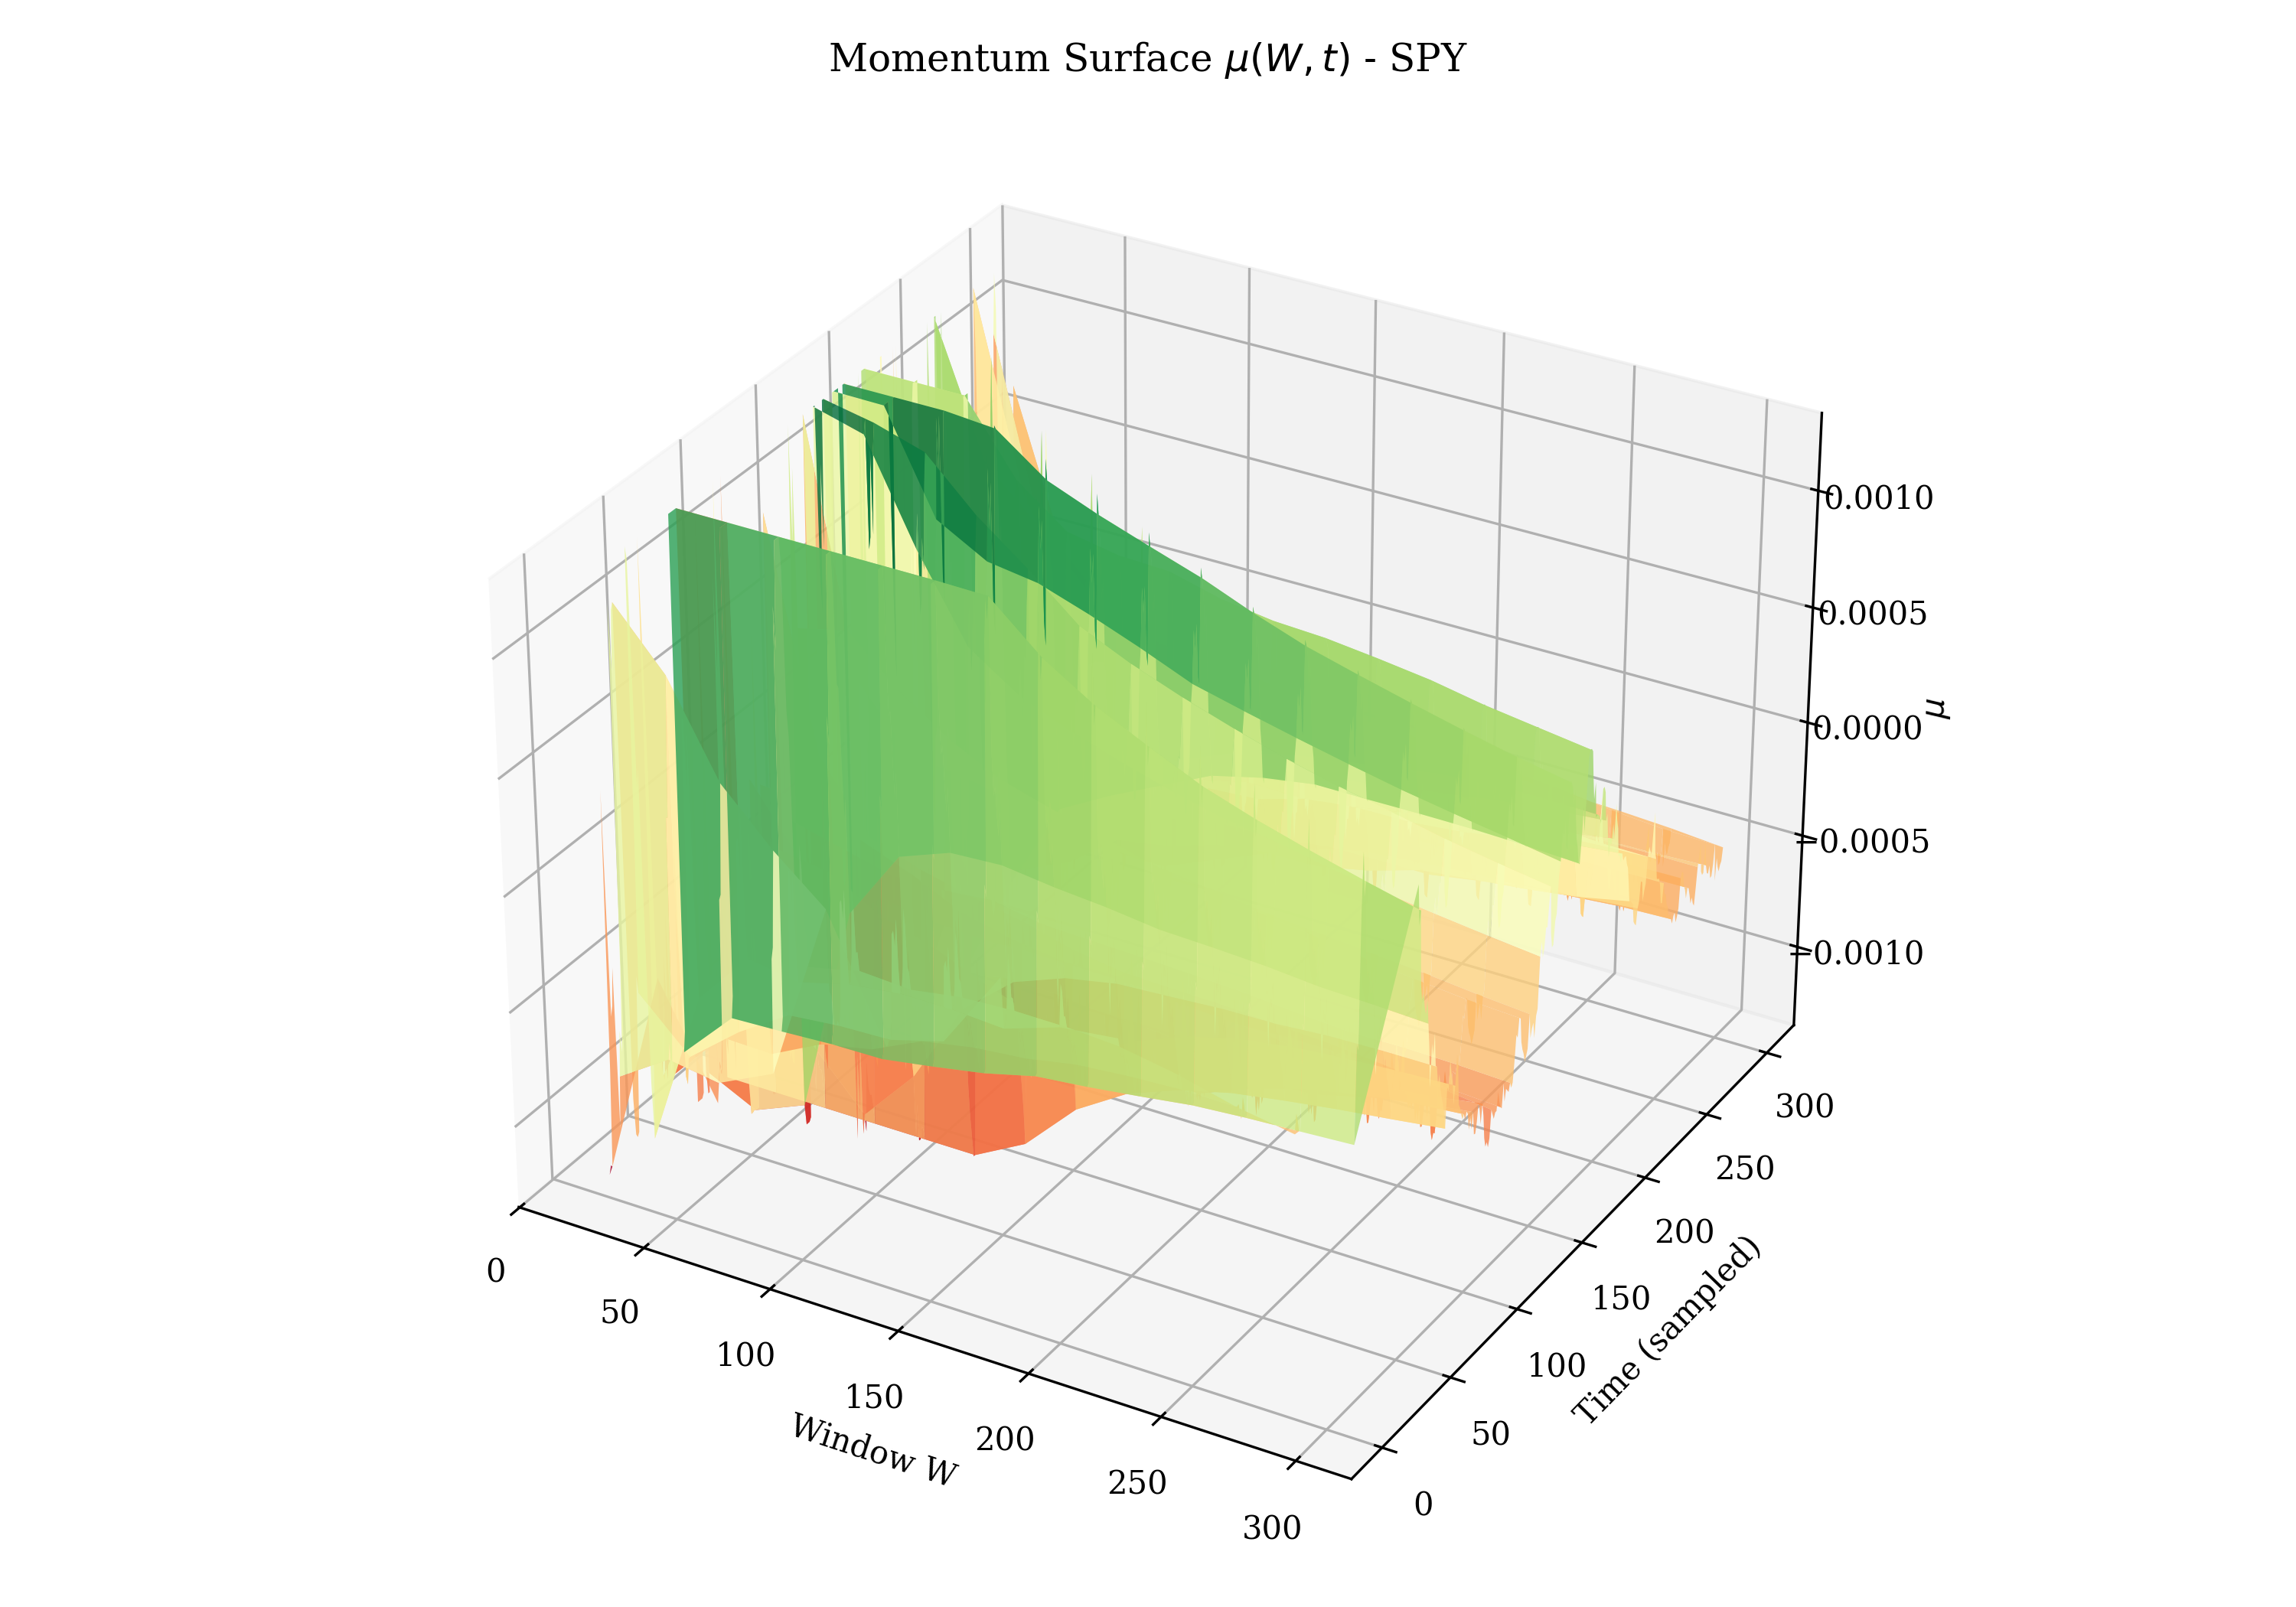
\includegraphics[width=0.7\textwidth]{images/spy_mu_surface.png}
    \caption{3D momentum surface $\mu(W,t)$ for SPY (2019--2025).}
\end{figure}

Evaluation is run on the frozen S\&P 500 ticker list (`data/sp500_tickers.txt`) from 2019-01-01 to 2025-01-01, with a chronological 70/30 train/test split. PMT performs a grid sweep over $W \in [20,300]$ (step 20) and $h \in [5,60]$ (step 5), selects $(W^*, h^*)$ on train, then reports both train and test Spearman correlations versus forward realized volatility. For direct model comparison, PMT and AR(1)-GARCH(1,1) are also compared at fixed horizons $h=\{10,21,31,42\}$.

\section{Results}
From 503 attempted tickers, both PMT and GARCH complete on 499. PMT's in-sample profile is still strong: mean $\rho_{train}=0.508$, median $\rho_{train}=0.531$. The distribution is shown in Figure 2.

\begin{figure}[ht]
    \centering
    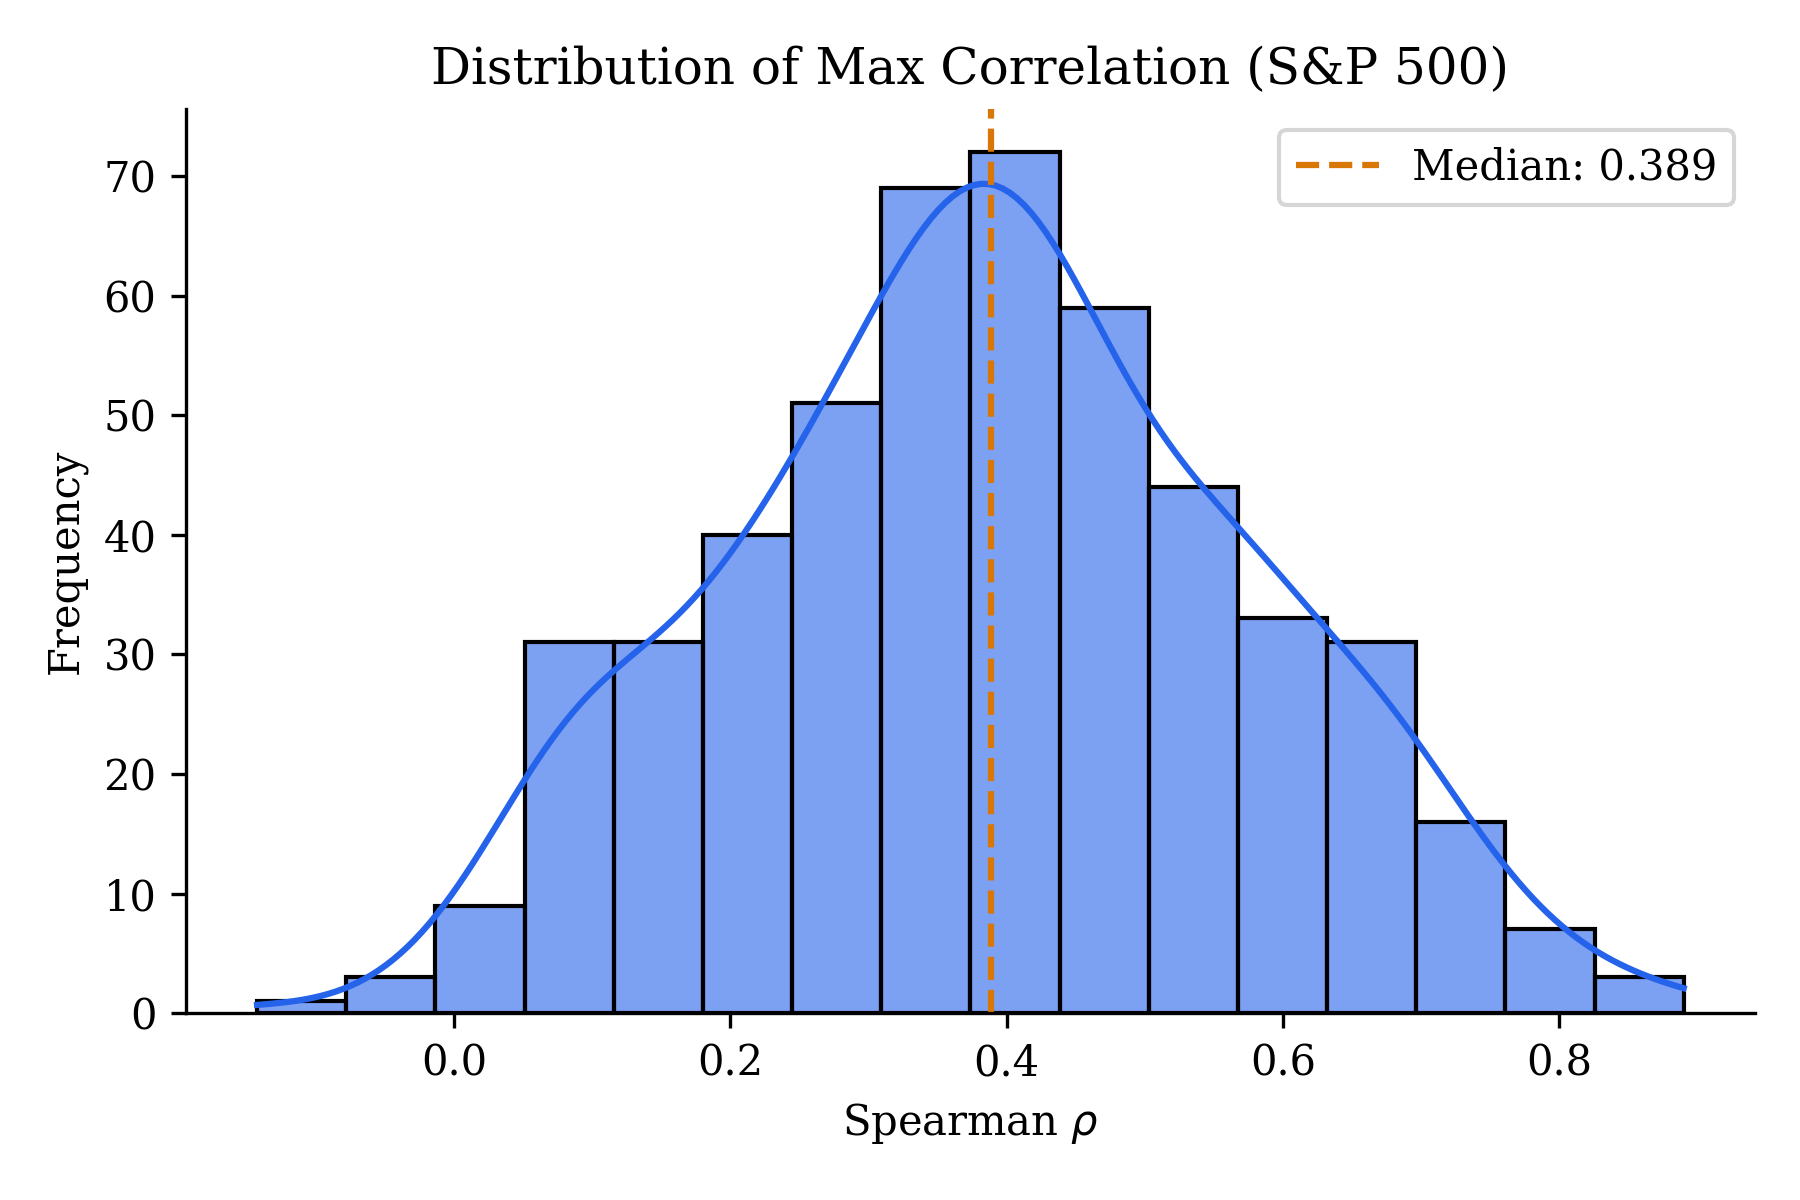
\includegraphics[width=0.6\textwidth]{images/rho_distribution.png}
    \caption{Distribution of PMT train-set max Spearman $\rho$ across S\&P 500 tickers.}
\end{figure}

Out-of-sample for per-ticker best parameters is much weaker: PMT reports mean $\rho_{test}=-0.018$ and median $\rho_{test}=0.010$ (491 non-null test observations). Parameter choices remain concentrated at long windows ($W^*$ mean 241.6, median 300) and long horizons ($h^*$ mean 43.1, median 60).

For apples-to-apples horizon comparison, results are more nuanced (Table 1). PMT has higher test \emph{median} rank correlation than GARCH at 10, 21, and 31 days, but lower test \emph{mean} at every reported horizon, and both metrics are weaker by 42 days.

\begin{table}[ht]
\centering
\caption{Out-of-sample horizon comparison (Spearman $\rho_{test}$ across 499 tickers).}
\begin{tabular}{lcccc}
\toprule
Horizon & PMT Mean & PMT Median & GARCH Mean & GARCH Median \\
\midrule
10 & 0.074 & 0.086 & 0.088 & 0.052 \\
21 & 0.069 & 0.061 & 0.081 & 0.033 \\
31 & 0.033 & 0.042 & 0.069 & 0.016 \\
42 & -0.003 & -0.002 & 0.063 & 0.011 \\
\bottomrule
\end{tabular}
\end{table}

SPY's surface-level behavior remains visually consistent with prior runs, with broad positive regions in the medium horizon zone and better stability at longer $W$.

\begin{figure}[ht]
    \centering
    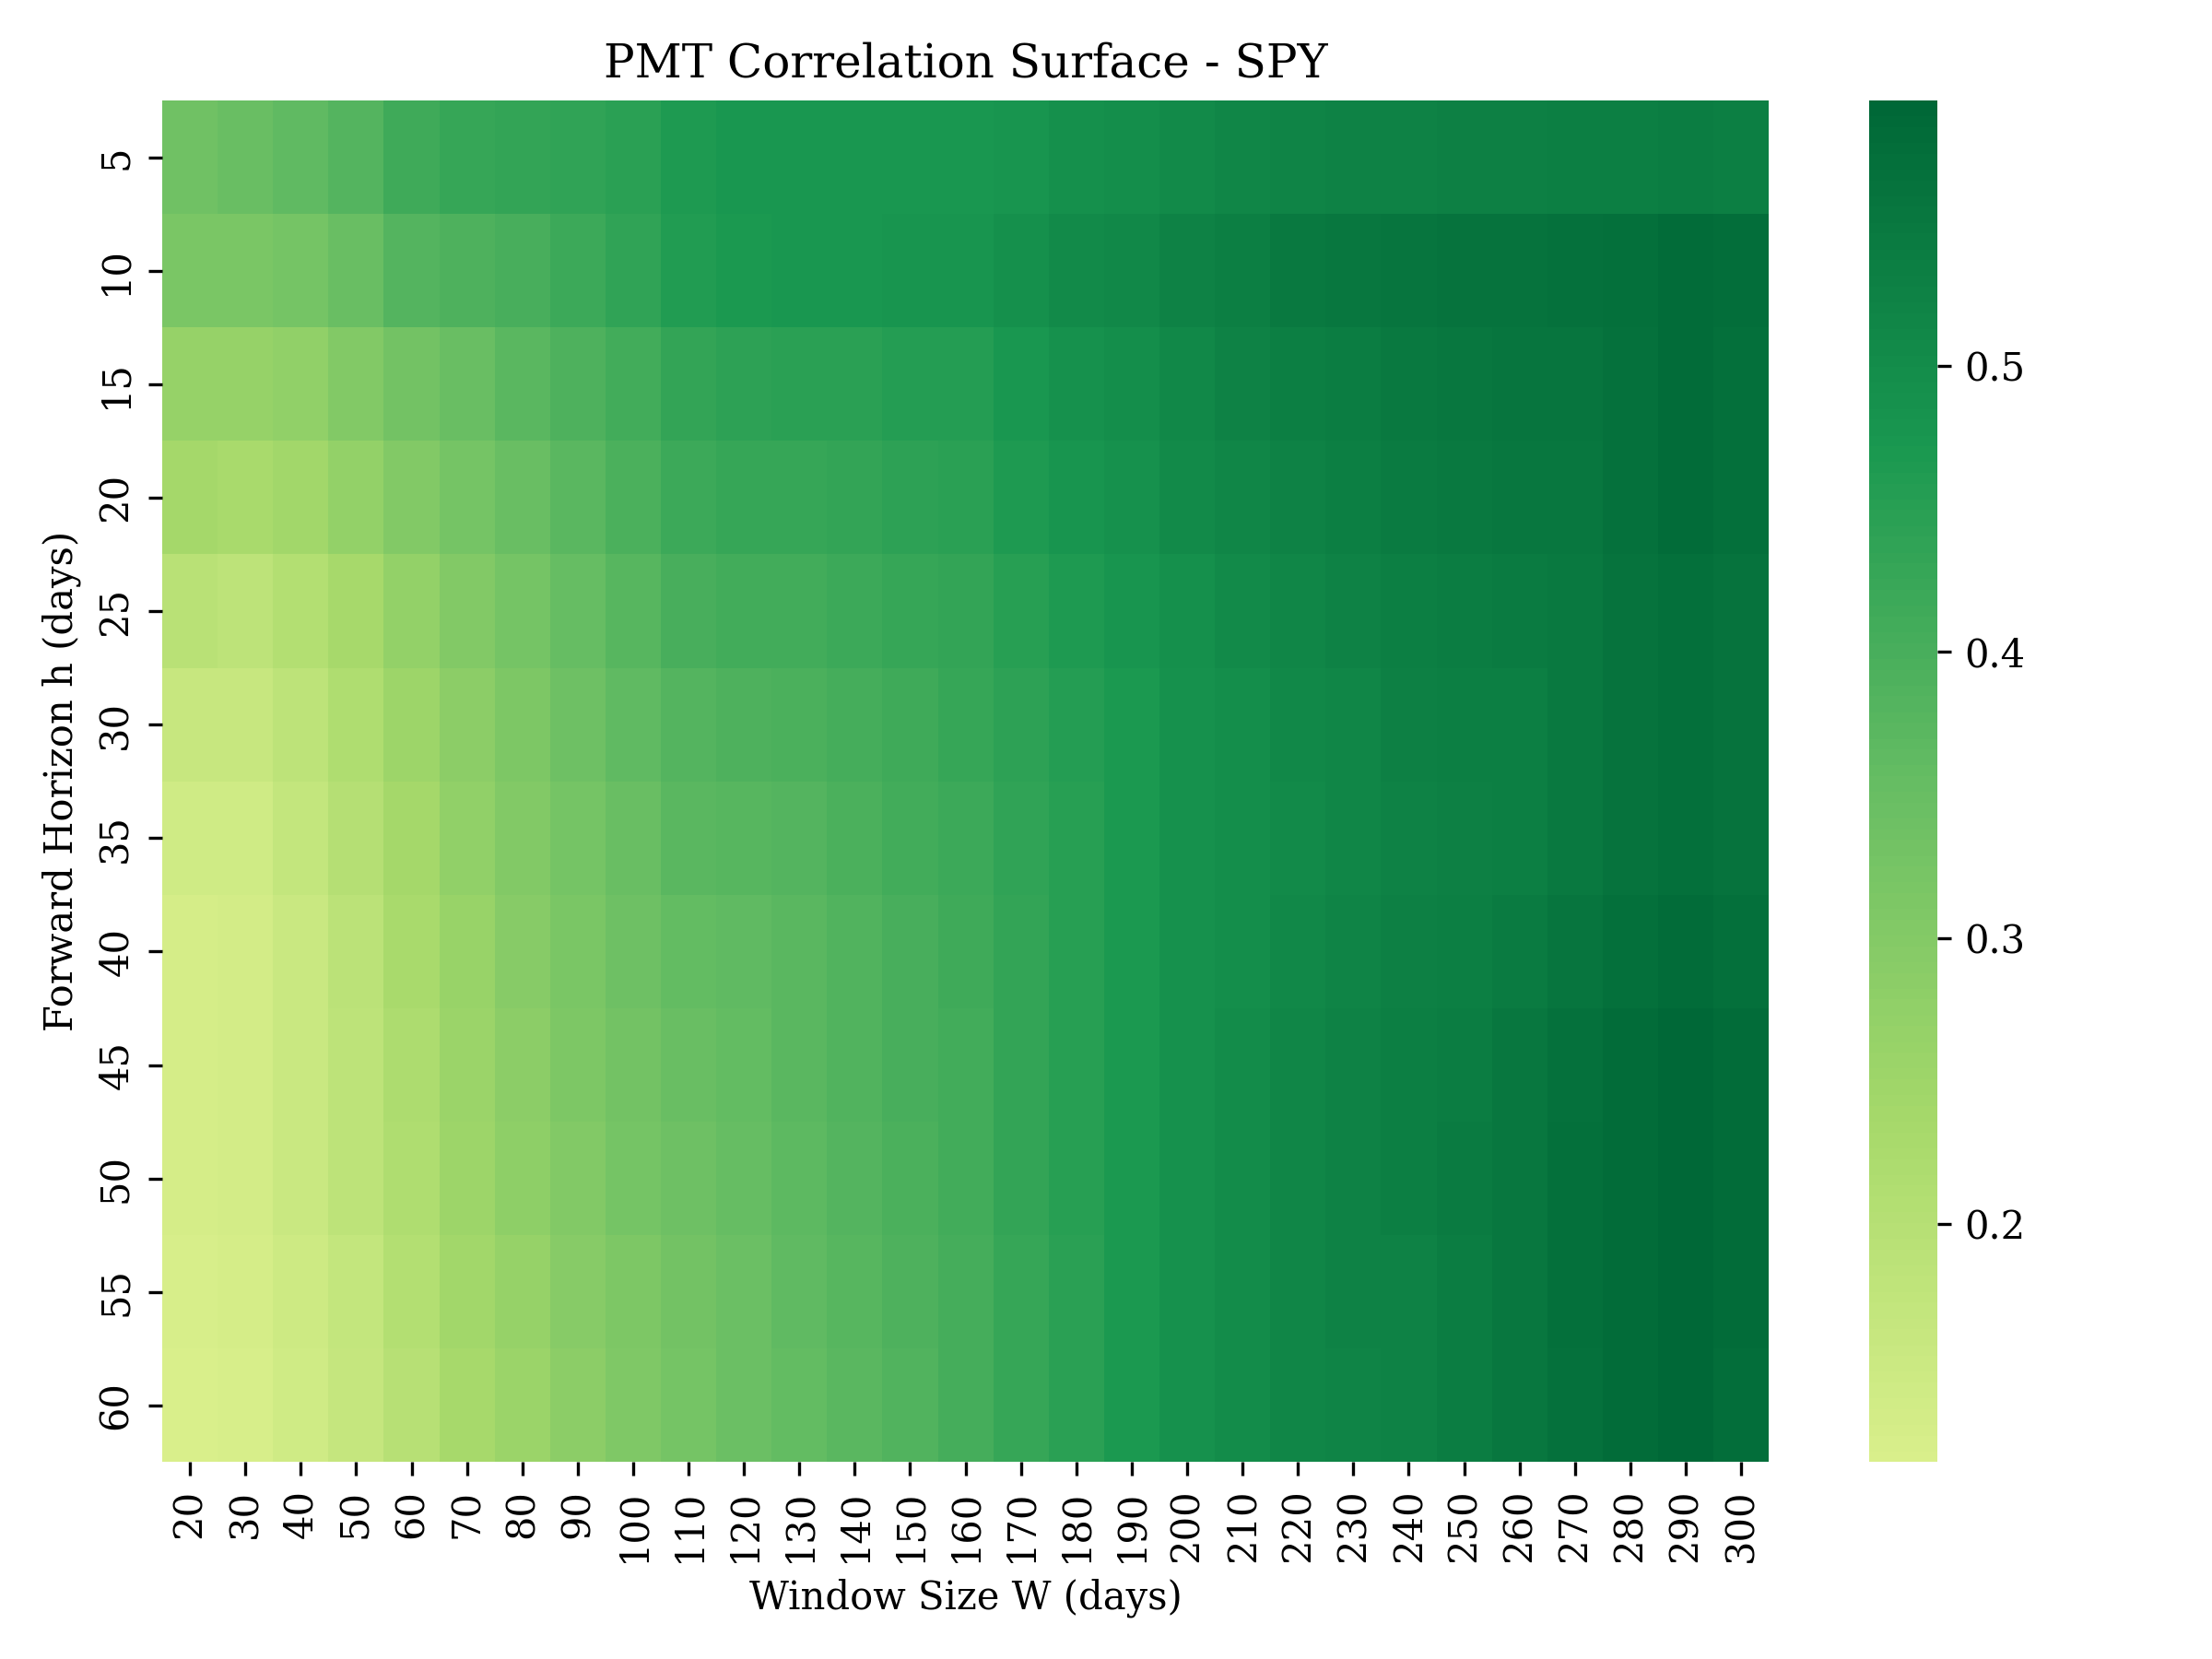
\includegraphics[width=0.6\textwidth]{images/spy_heatmap.png}
    \caption{Spearman correlation surface for SPY (2019--2025).}
\end{figure}

\section{Discussion}
Short version: the signal is real, but not magic. PMT crushes in-sample and still has useful out-of-sample behavior at short to medium horizons, especially if you judge robustness with medians. But once we demand broad out-of-sample consistency across the full cross-section, performance compresses hard and can flip negative at longer forecast horizons.

So the practical read is straightforward and professional:
\begin{itemize}
    \item PMT should be treated as a horizon-aware feature, not a one-number universal forecaster.
    \item Cross-sectional tails matter; means and medians can disagree, and both should be reported.
    \item GARCH remains a competitive baseline, especially for longer horizons where PMT signal decays.
\end{itemize}

In other words, PMT is still useful, but deployment should probably be ensemble-first (PMT + volatility-model baseline), with strict walk-forward validation and horizon-specific calibration.

\section{Conclusion}
PMT remains a compelling structural-volatility signal when evaluated carefully. The updated repository results support a balanced claim: strong in-sample ranking power, mixed but non-trivial out-of-sample utility at shorter horizons, and clear degradation as horizon extends. The framework is worth advancing, but the next step is disciplined model governance: rolling retraining, stability filters on $(W^*,h^*)$, and combination with established volatility models rather than replacing them outright.

\vspace{1em}
\noindent \textit{Note: all numbers in this report are taken from the checked-in CSV and manifest artifacts in `results/`.}

\end{document}
